\documentclass[12pt]{article}
% Margin fixes
\oddsidemargin -0.5in
\evensidemargin -0.5in
\textwidth 7.25in
\topmargin 0.0in

\headheight 0.0pt
\headsep 0.0pt
\voffset 0.0pt
\textheight = 9.0in
\usepackage{amsmath,amssymb,graphicx,float}

\title{Seismometer}
\author{Nathan Grouse\\Lisa Tran}

\newcommand{\eV}{\text{eV}}
\newcommand{\V}{\text{V}}
\newcommand{\A}{\text{A}}

% Start the document!
\newcommand{\documentname}{\textsl{Article}}
\begin{document}
\maketitle

\section{Introduction}
\indent \indent A pendulum seismometer with damping magnets can be used to evaluate different quality factor values for different positions of the magnets, and detect and analyze subways passing under the building.

\subsection{Apparatus}
\indent \indent The seismometer consists of a swinging arm and a suspension arm, both attached to pivots and the rest of the apparatus. The rest of the apparataus consists of a mass, a coil that senses movement of that mass, a damping plate, and adjustable damping magnets. The entire apparatus is surrounded by a plastic screen / box so that the pendulum isn't affected by motion in the room.

\begin{figure}[H]
\centering
\hspace{-0.0in}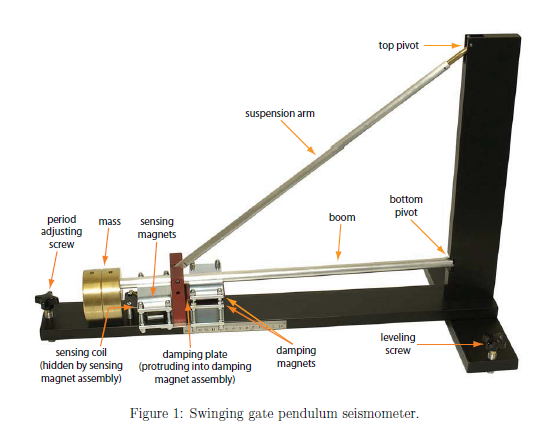
\includegraphics[scale=0.90]{apparatus.png}
\end{figure}

\section{Theory}
\indent \indent The lecture notes are very detailed.

\section{Data}
\begin{figure}[H]
\centering
\hspace{-0.0in}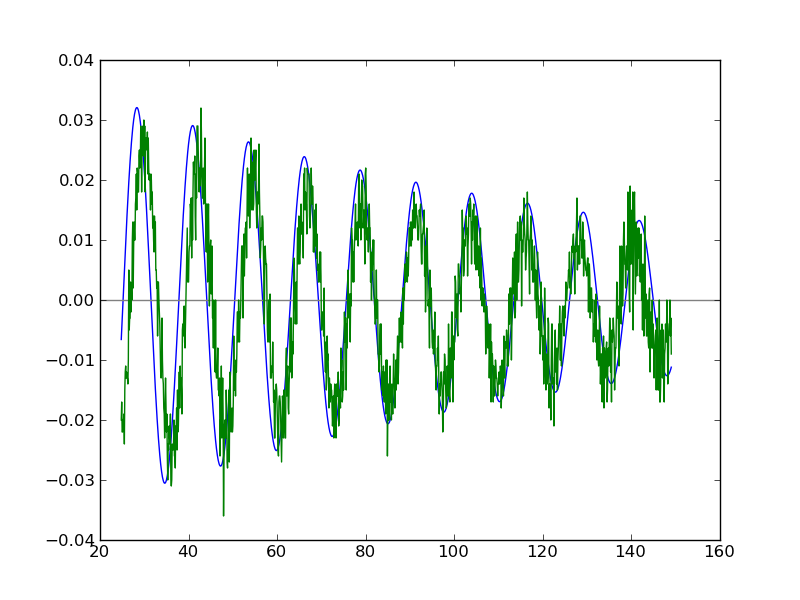
\includegraphics[scale=0.60]{SeisPosition1.png}
\caption{Position: Furthest from the mass, Q = 32. \label{fig:setup}}
\end{figure}

\begin{figure}[H]
\centering
\hspace{-0.0in}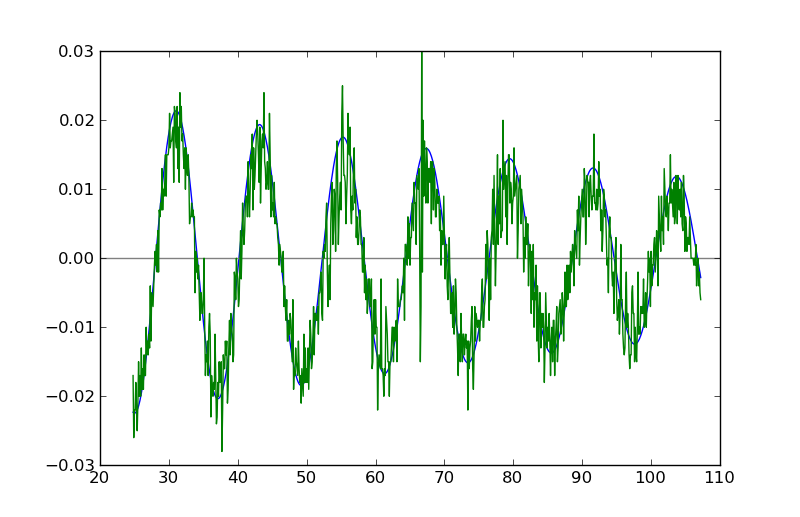
\includegraphics[scale=0.60]{SeisPosition2.png}
\caption{Position: 0 cm, Q = 32. \label{fig:setup}}
\end{figure}

\begin{figure}[H]
\centering
\hspace{-0.0in}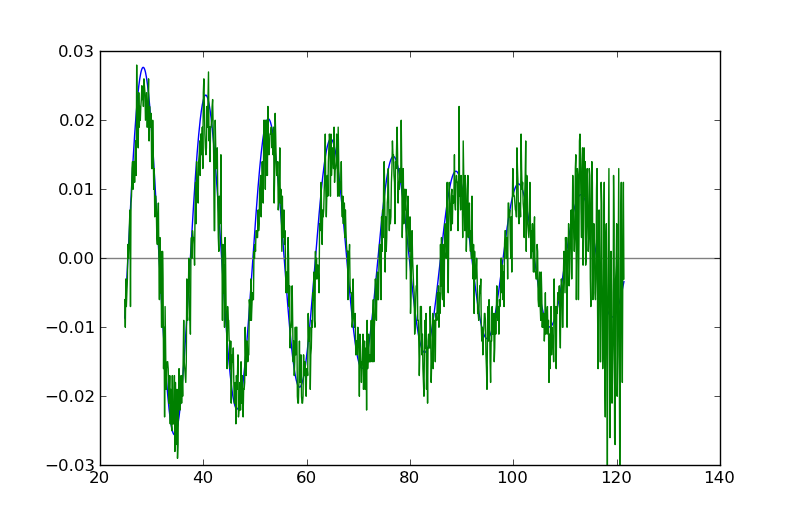
\includegraphics[scale=0.60]{SeisPosition3.png}
\caption{Position: 5 cm, Q = 20. \label{fig:setup}}
\end{figure}

\begin{figure}[H]
\centering
\hspace{-0.0in}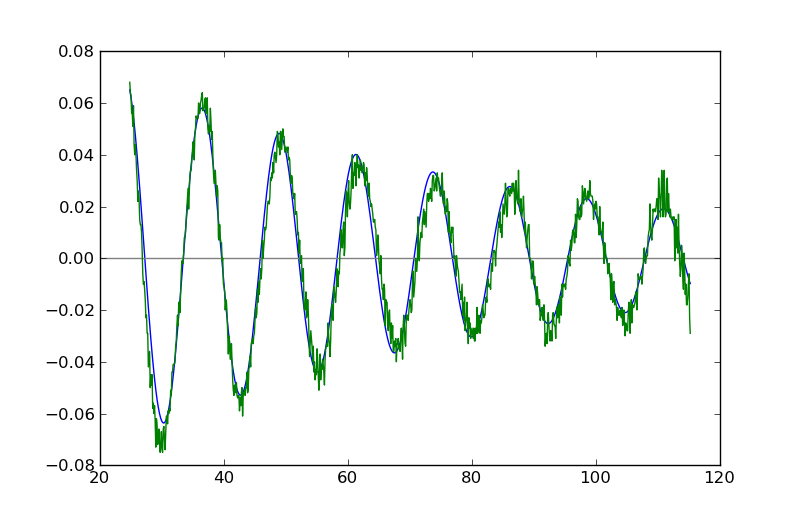
\includegraphics[scale=0.60]{SeisPosition4.png}
\caption{Position: 8 cm, Q = 17. \label{fig:setup}}
\end{figure}

\begin{figure}[H]
\centering
\hspace{-0.0in}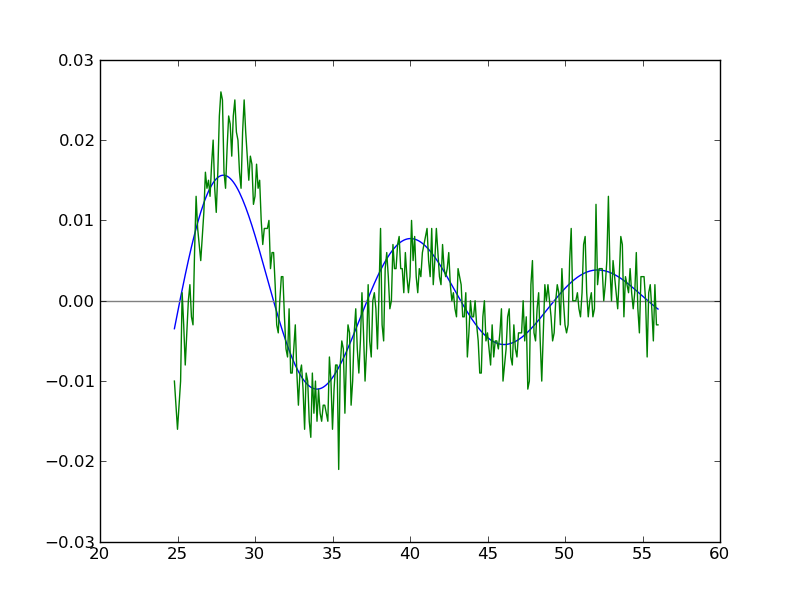
\includegraphics[scale=0.60]{SeisPosition5.png}
\caption{Position: 9.4 cm, Q = 4.5. \label{fig:setup}}
\end{figure}

\begin{figure}[H]
\centering
\hspace{-0.0in}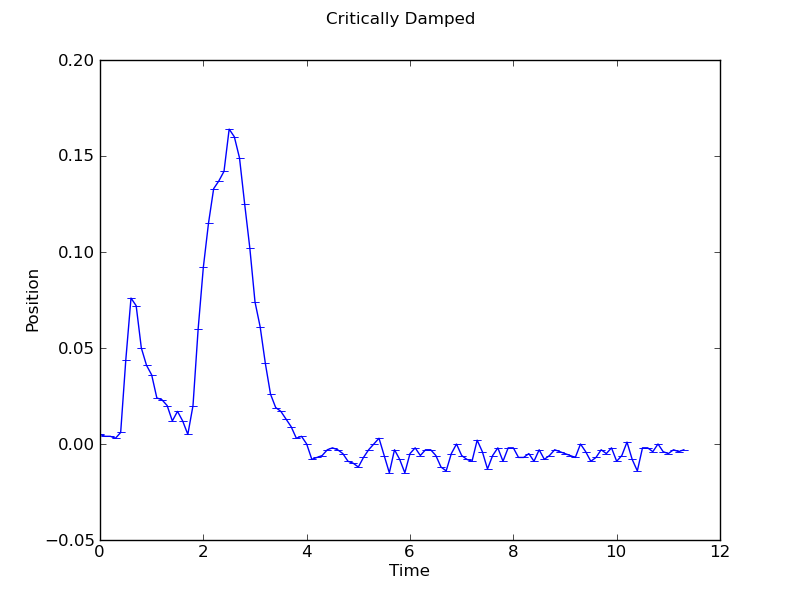
\includegraphics[scale=0.60]{SeisPosition6.png}
\caption{Position: 12.0 cm, Q = 0.5. \label{fig:setup}}
\end{figure}

\begin{figure}[H]
\centering
\hspace{-0.0in}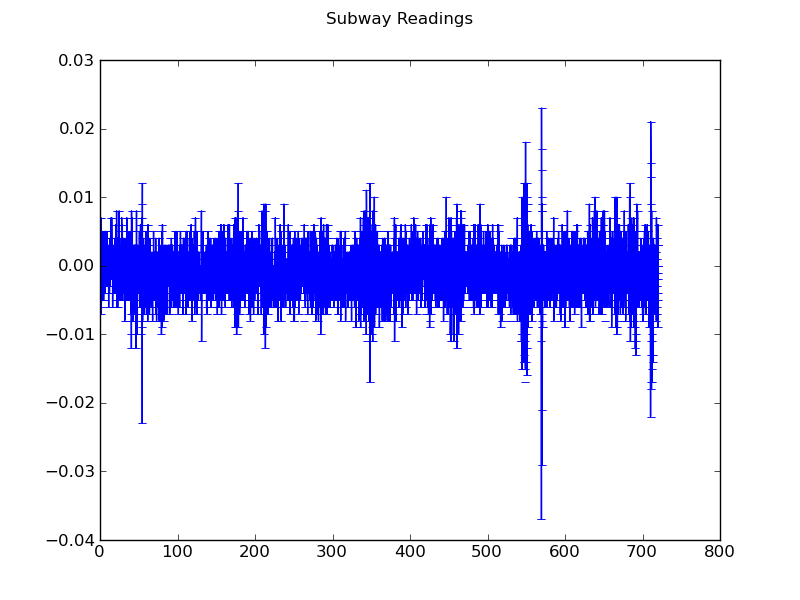
\includegraphics[scale=0.60]{Subway.png}
\caption{This data was not very readable when plotted with python. \label{fig:setup}}
\end{figure}

\begin{figure}[H]
\centering
\hspace{-0.0in}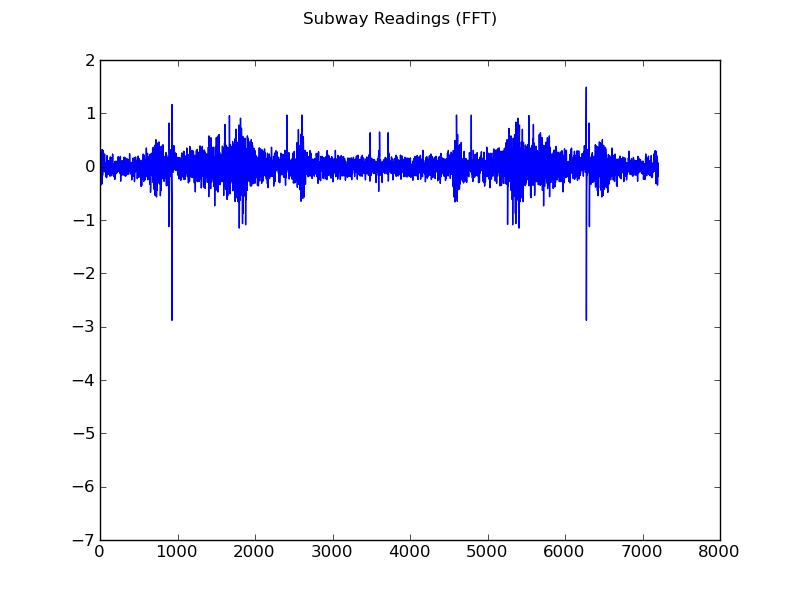
\includegraphics[scale=0.60]{SubwayFFT.png}
\caption{This data was not very readable when plotted with python. \label{fig:setup}}
\end{figure}

\section{Error Analysis}
\indent \indent There was uncertainty in our readings determined by the sensing coil. This uncertainty, important in its implication that any measurement has some level of uncertainty, will not be used for any calculations.

\section{Conclusion}
\indent \indent "Calculations" were done with python by changing parameters in a program to fit an exponentially decaying sinusoidal wave to the data gathered for the experiment. This lab was meant to show how changing damping physically will affect the quality factor, where the quality factor is determined using the python program. We were also meant to analyze the affects of the NYC subway system on our pendulum seismometer, but the data was not well recieved by my python plotting software. The data recieved for the subway was put through a FFT built into the data gathering program and we were meant to determine the characteristic frequency of the subway and amplitudes of accelerations, velocities, and displacements of the building. When I tried to put my data through Scipy's FFT function, nothing useful happened.

\section{Questions}
\indent \indent 1. What quantity does the pick-up coil measure and exactly what quantity or quantities is the isntrument sensitive to? \\
\indent The coil measures changes in voltage as determined by motion in the pendulum, specifically at the mass.\\
\indent 2. What are the characteristic frequencies of the vibrations? \\
\indent I can't determine that.\\
\indent 3.Repeat your measurements both with and without the vibration isolation mounts for the wooden table. Do you see a difference? \\
\indent We did not complete this part of the experiment. I would expect the apparatus to be more sensitive to the vibrations in the room - footsteps, leaning on the table, doors slamming, etc. - and the vibrations from the subway.

\end{document}